\section{Test the IDE with Hello World}
\label{sec.hello.world}

The first program we usually write in any programming language is
called \code{hello-world}.  It is a very simple program.  However
getting it to run means you have to understand how to use the
programming environment.

\subsection{Examine the Hello World Code}
\label{sec.examine.the.code}
\begin{enumerate}
\item Take a look at the Python code in the file \code{src/hello.py}. 

\item Find the declarations of the function named \code{hello} and
 \code{hello\_pierre}, as shown in Listing~\ref{list.hello}.

\begin{listing}{Declaration and Use of Function \code{hello}}{hello}
\begin{minipage}[c]{0.95\textwidth}\begin{lstlisting}
def hello(name):
    return ("Hello, " + name + "!")

def hello_pierre():
    # CHALLENGE: student must complete the implementation.
    raise NotImplementedError()
\end{lstlisting}\end{minipage}\end{listing}

\item Your task it to replace \code{raise NotImplementedError()} with correct python code.

\item Two conditional calls to the function \code{hello}, each time
  with a different argument, shown in Listing~\ref{list.calls}.


\begin{listing}{Calls to Function \code{hello}}{calls}
\begin{minipage}[c]{0.95\textwidth}\begin{lstlisting}
if __name__ == '__main__':
    # call the function with an argument
    print(hello("gertrude"))
    
    # second test
    print(hello("fred"))

    # Follow the two examples above. Add a line
    #   so that Python will print a hello message 
    #   to pierre.
    # CHALLENGE: student must complete the implementation.
    raise NotImplementedError()
\end{lstlisting}\end{minipage}\end{listing}




\item Find the icon \includegraphics[height=1.0cm]{run-triangle.png} in the
top-right of the editor window.  Click the triangle, to see a sample
run/execution of the code.

\noindent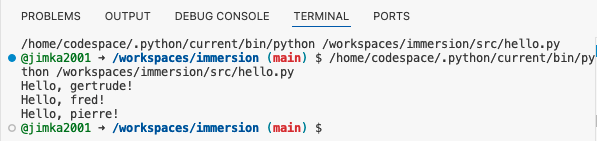
\includegraphics[width=\textwidth]{hello-terminal-output.png}

\end{enumerate}

\subsection{Running Predefined Tests}
\label{sec.run.tests}
\begin{enumerate}


\item Open the file \code{tests/test\_hello.py} in a GitHub Code-Space.

\noindent\includegraphics[width=0.4\textwidth]{test-hello-explorer.png}

\item To run the tests, press the
\includegraphics[width=1cm]{run-triangle.png} which you should find in
the upper-right corner of the editor window.

\noindent\includegraphics[width=0.8\textwidth]{hello-test.png}


\item The text window at the bottom of the editor should show the results of
how many tests ran and whether there are any failures.

\noindent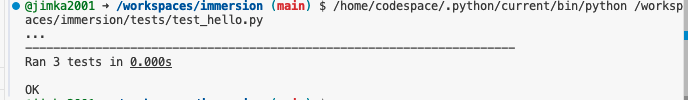
\includegraphics[width=0.9\textwidth]{github-test-result.png}

\item If some of the tests fail, try to understand the error message, and edit
  the code in \code{hello.py} and try again until the tests pass.  There are many
  different ways test might fail.  The following is one example of possibly many.

\noindent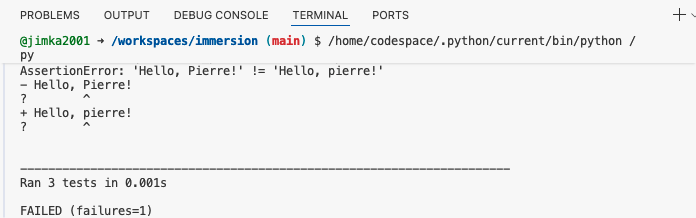
\includegraphics[width=0.9\textwidth]{tests-fail.png}


\end{enumerate}

\clearpage

% LocalWords:  GitHub png github
